\section{Iteration 2: Decomposition of the Remote Module Communication Unit}
\label{add:it2}

\subsection{Step 1: Identify candidate drivers}
\label{add:it2/drivers}

\npar In the previous iteration, four quality attributes (Av2', M1', M2' and
M3') and three use cases (UC7, UC8' and UC13') were assigned to the remote
module communication unit and one use case (UCy) was derived. 

\npar The decomposition is entirely driven by the quality attribute scenarios. 

\begin{itemize}
  	\item Av2': Missing measurements
  	\begin{itemize}
    	\item When a measurement did not arrive this should be logged, when
  		this happens for the third time, a ReMes Operator should be notified. This
  		detection should occur in less than ten minutes.
		\item Trames should be resent when they are not acknowledged.
  	\end{itemize}
  	\item M1': Dynamic pricing
  	\begin{itemize}
    	\item New types of remote devices will be introduced (with possibly new
    	data formats of the trames they send).
  	\end{itemize}
  	\item M2': Fine-grained metering for enterprises
  	\begin{itemize}
    	\item The secondary meters can introduce new trame formats
  	\end{itemize}
  	\item M3': Decentralized electricity generation
  	\begin{itemize}
   		\item The production meters could define a new trame format
  	\end{itemize}
\end{itemize}

\npar The use cases delegated to this unit are given below.

\begin{itemize}
	\item UC7: Send trame to remote device
	\item UC8': Send measurement
	\begin{itemize}
	    \item Incoming trames are acknowledged.
    	\item Remote modules are marked as active when they send their first trame.
  	\end{itemize}
  	\item UC13': Send alarm
  	\begin{itemize}
		\item The incoming trame should be acknowledged
		\item Possibly, a control trame will be sent to shut a valve
  	\end{itemize}
  	\item UCx: Retrieve customer from trame
  	\item UCy: Retrieve remote module protocol
\end{itemize}

\subsection{Step 2: Choose design concepts}
\label{add:it2/concepts}

\subsubsection{Tactics}
\label{add:it2/tactics}

\paragraph{Modifiability}

\npar When opting for a modifiable solution three main (groups) of tactics can
be used: localize modifications, prevent ripple effect and defer binding time.
Two tactis are picked from the first group, namely abstraction of common
services and anticipate expected changes.

\npar To prevent rippling effects three tactics are employed. The first one,
probably the most important one, is the hiding of information through the use of
interfaces. Furthermore are communication paths restricted and an intermediary
will be used.

\paragraph{Availability}

\npar The chosen availability tactic is detection, more specific the heartbeat
mechanism.

\subsubsection{Design Patterns}
\label{add:it2/patterns}

\npar To realize the modifiability tactics and allow the coverage of UC7', the
\emph{Message Translator} pattern \citep[see][p.~229]{Buschmann:07} and the
Layers design pattern \citep[see][p.~185]{Buschmann:07} are selected.
The translator acts an intermediary between the remote module and ReMeS and all
information remains hidden behind a simple interface.

\npar To push this information hiding even further a modified version of the
\emph{Resource Pool} pattern is used. This will be enlightened in the next
section.
%TODO: misschien is dit niet helemaal waar, want resource pool is meer op
% performantie gericht.

\npar Finally the \emph{Publisher-Subscriber} pattern
\citep[see][p.~234]{Buschmann:07} is used to allow multiple components to
receive trames in parallel.

\subsection{Step 3: Instantiate architectural elements and allocate responsibilities}
\label{add:it2/elements}

\begin{figure}[H]
	\begin{centering}
		% TODO Figure
		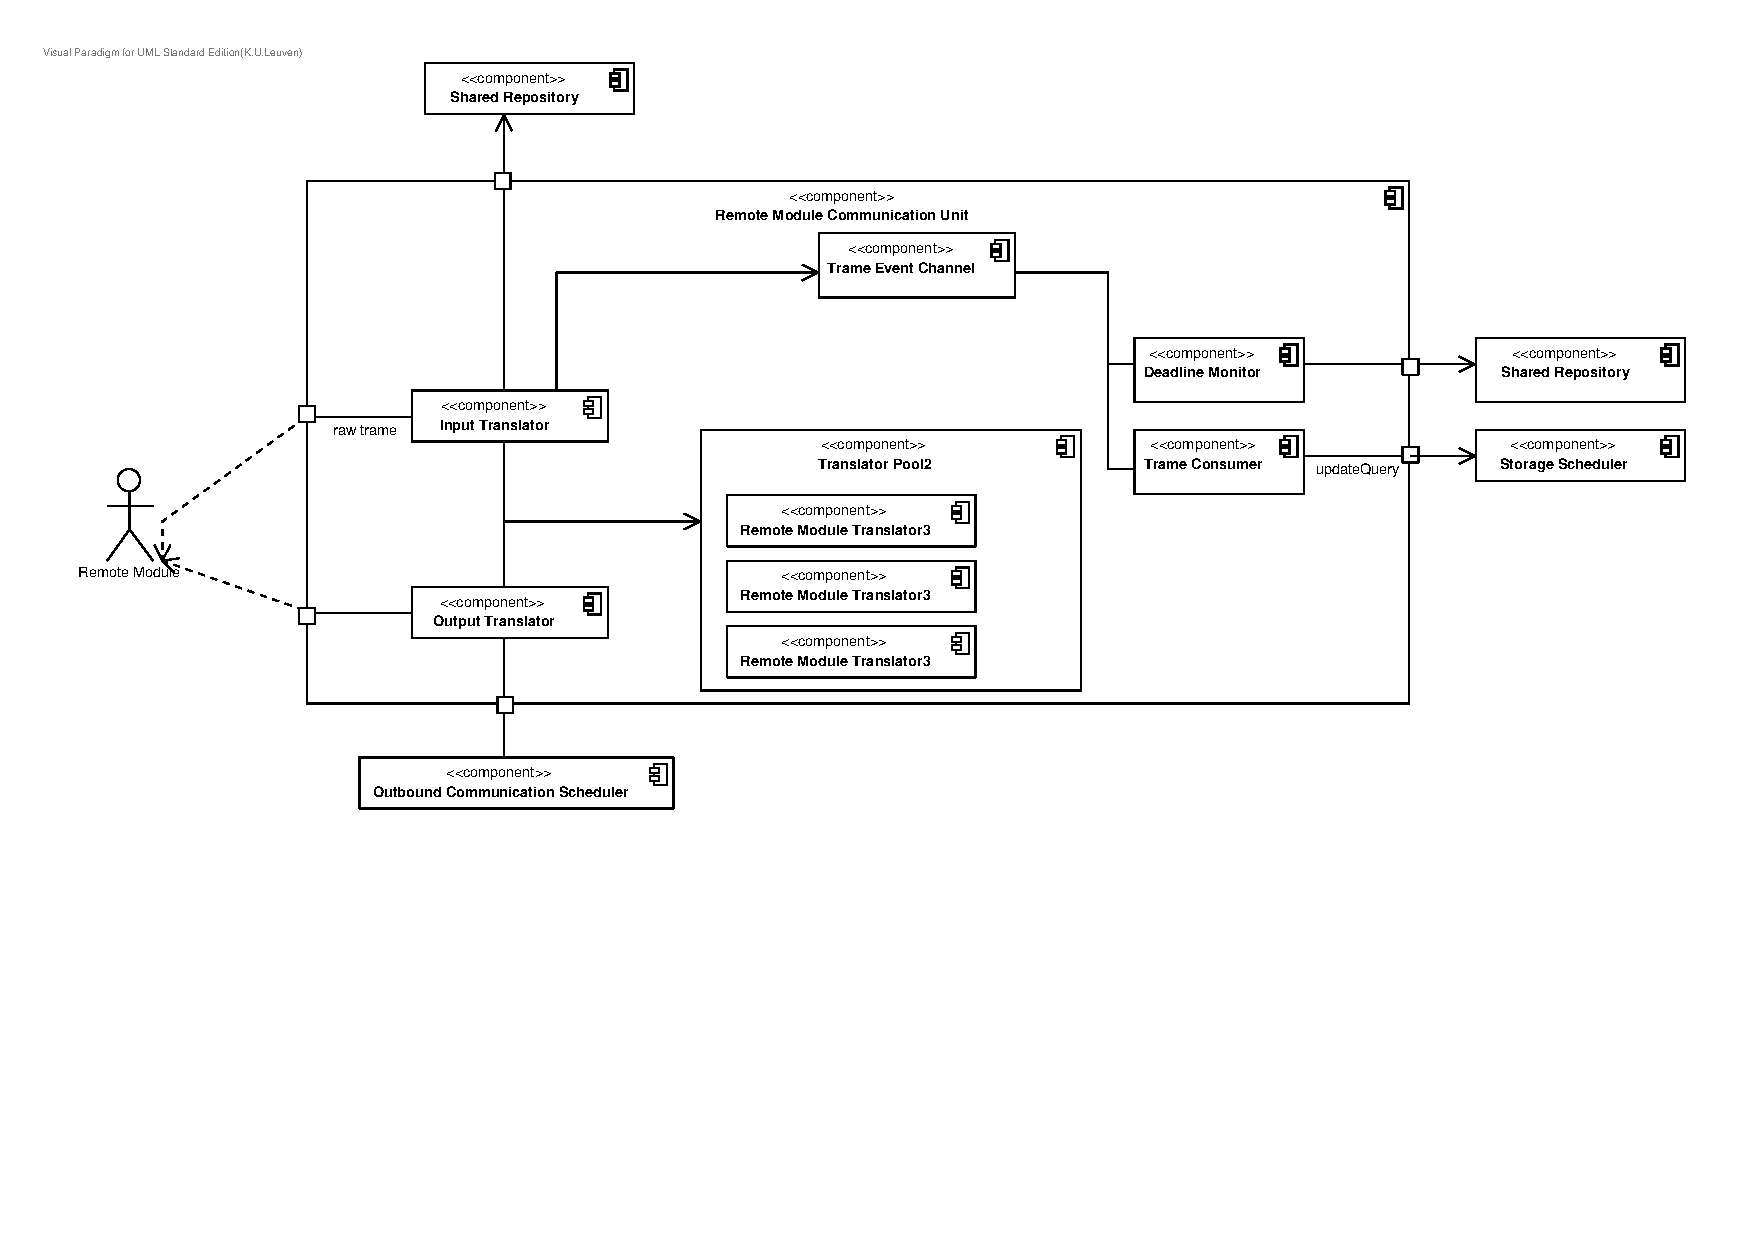
\includegraphics[width=\textwidth]{figs/add-it2-elements.pdf}
		\caption{Overview of the instantiated child elements in the Remote Module
		Communication Unit}
		\label{fig:it2/elements}
	\end{centering}
\end{figure}

\npar The remote module communication unit has six main components: Input
Translator, OutputTranslator, TranslatorMap, TrameEventChannel, DeadlineMonitor
and TrameConsumer. Each of them will be discussed below. As one can see in
diagram \ref{fig:it2/elements} there are only two communication paths in the
system, one for incoming communication and one for outgoing. In this way another
tactic is realized, namely the restriction of communication paths.
% TODO: is die restriction tactic nog wel valid ? sloeg op een (veel) eerder
% design

\npar In the previous section there was the mentioning of a modified version of
the \emph{Resource Pool} pattern. One can see this pattern in the usage of the
TranslatorMap. The TranslatorMap component itself acts as a sort of manager of
the map and handles incoming requests for translators based on a certain module.
The difference with the original pattern lies in the diversity of the
translators. Each translator is different whereas the resources normally should
all be equal.

\subsubsection{InputTranslator}

\npar The InputTranslator has as duty the translation of incoming (raw) trames
into objectified trames. Therefore it must know what the incoming data format
is. To realize this, it has a TranslatorMap at its disposal where, based on
the module (type) a RemoteModuleTranslator can be fetched. When the trames are
translated they are published on the event channel for all interested parties.

\subsubsection{OutputTranslator}

\npar This component is analogous to the InputTranslator off course. This
component retrieves the right RemoteModuleTranslator from the map based on the
module where the incoming trame should be send to. It is important to notice that all
outgoing communication towards remote modules goes through this module.

\subsubsection{TranslatorMap}

\npar The TranslatorMap acts as the manager for the map and all requests from
both the translators will pass through this component. 

\subsubsection{TrameEventChannel}

\npar The event channel is the communication entity where publishers can publish
events on and subscribers can subscribe on. In this context the InputTranslator
will publish events on the channel. The subscribers are the DeadlineMonitor and
the TrameConsumer.

\subsubsection{DeadlineMonitor}

\npar The responsibility of this component is the monitoring of all bypassing
measurements and guaranteeing that a missing measurement is detected within the
demanded time limits. This monitor is subscribed to the event channel to receive
trames. To guarantee these limits the monitor keeps a table with expected
arrival times of all remote devices which is frenquently checked. To constrcut
the table the shared repository is contacted to retrieve the send frequency of
each of the modules. Notice that to protect from failures, this table is made
persistent. When a deadline is exceeded this is stored in the corresponding
database. When a certain number of deadline violations is reached a ReMeS
operator is notified. Notice that this component is in fact the realization of
the heartbeat tactic.

\subsubsection{TrameConsumer}

\npar The trame consumer is a forwarding unit which is subscribed to the event
channel and receives all events which are published on it. It converts all
measurements into insert queries which are to be scheduled on the
measurement scheduler. Alarms are converted into commands and they are
subsequentely sent to the anomaly scheduler. So this component is at the same
time a router and a translator.

\subsection{Step 4: Define interfaces for instantiated elements}
\label{add:it2/interfaces}

\npar In this section each interface is explained in terms of the components
which use and/or offer it together with information about what is exchanged. For
detailed information with reference to the specific methods the interfaces
implement, we refer to the interface catalog, see appendix
\ref{chap:interface-catalog}.

\subsubsection{InboundCommAPI}

\npar this interface was already discussed in iteration 1, see section
\ref{add:it1/interfaces}.

\subsubsection{OutboundCommAPI}

\npar this interface was already discussed in iteration 1, see section
\ref{add:it1/interfaces}.

\subsubsection{TranslatorManager}

\npar This interface lies in between the InputTranslator and OutputTranslator
on one side and the TranslatorMap, who implements it, on the other side.
Through this interface translators are passed.

\subsubsection{Translator}

\npar Each of the different translators implements the \interface{Translator} 
interface. The users of this interface are the aforementioned input and output
translator.

\subsubsection{TrameChannel}

\npar This interface lies in between the trame event channel and its users
(i.e. publishers and receivers). Events flow through the channel, originating at
a publisher and ending at one or more subscribers.

\subsubsection{CommEventNotifiable}

\npar This interface complements the \interface{TrameChannel} interface. When a
component is subscribed to a certain event flow, the channel has to be able to
notify the component when a new event is available. This is done through this
interface which is implemented by subscribers (in this context deadline monitor
and trame consumer).

\begin{figure}[H]
	\begin{centering}
		% TODO Figure
		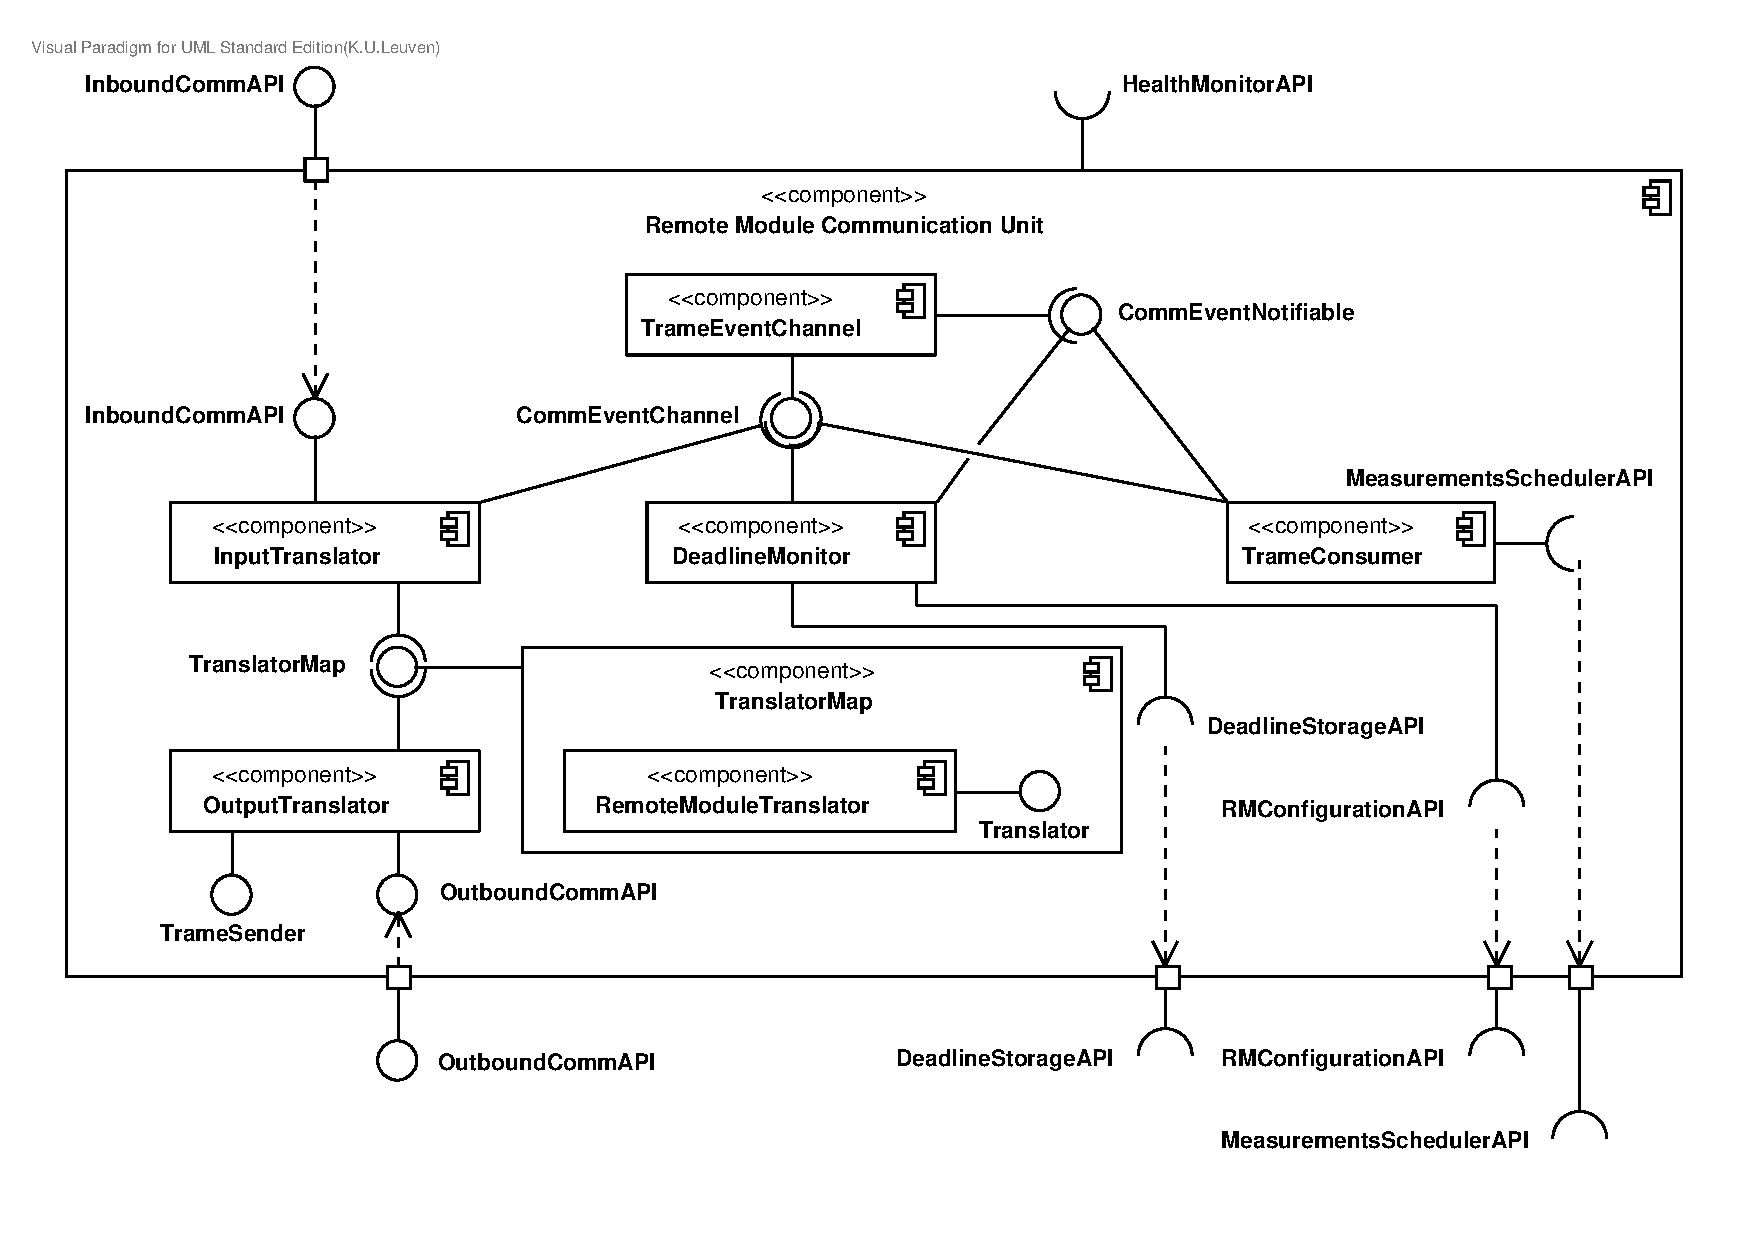
\includegraphics[width=\textwidth]{figs/add-it2-interfaces.pdf}
		\caption{Overview of the interfaces and components in the remote
		module communication unit}
		\label{fig:it2/interfaces}
	\end{centering}
\end{figure}

\subsection{Step 5: Verify and refine}
\label{add:it2/verification}

\npar All quality requirements are resolved in this iteration so no futher
decomposition of any of the child modules have to take place. The use cases
are delegated to child elements. 

\begin{itemize}
	\item UC7: Send trame to remote device. The OutputTranslator has to take care
	of this. 
  	\item UC8': Send measurement. The acknowledgement of incoming trames will
  	be handled by the InputTranslator. New remote devices are marked active by
  	the TrameConsumer. 
  	\item UC13': Send alarm. The acknowledgement of trames is already implemented
  	in UC8' and as such it is taken care of.
  	\item UCy: Retrieve remote module protocol. This functionality applies to
  	both the InputTranslator and OutputTranslator. 
\end{itemize}
